%!TEX root = CVPR_2018_Nonlinear_3DMM.tex
\Section{Proposed Method}
\label{sec:alg}

\SubSection{Conventional Linear 3DMM}
The 3D Morphable Model (3DMM)~\cite{blanz1999morphable} and its 2D counterpart, Active Appearance Model~\cite{cootes2001active,face-model-fitting-on-low-resolution-images}, provide parametric models for synthesizing faces, where faces are modeled using two components: shape and texture. 
In~\cite{blanz1999morphable}, Blanz et al.~propose to describe the 3D face space with PCA:
\begin{equation}
\mathbf{S} = \mathbf{\bar{S}} +  \mathbf{A} \mathbf{\alpha},
\eqnvspace
\end{equation}
where $\mathbf{S}\in\mathbb{R}^{3Q}$ is a 3D face with $Q$ vertices, $\mathbf{\bar{S}}\in\mathbb{R}^{3\times Q}$ is the mean shape, $\alpha\in\mathbb{R}^{l_S}$ is the shape parameter corresponding to a 3D shape bases $\mathbf{A}$. 
%
The shape bases can be further split into $\mathbf{A} = [\mathbf{A}_{id}, \mathbf{A}_{exp}]$, where $\mathbf{A}_{id}$ is trained from 3D scans with neutral expression, and $\mathbf{A}_{exp}$ is from the offsets between expression and neutral scans.

The texture $\mathbf{T}^{(l)}\in\mathbb{R}^{3Q}$ of the face is defined within the mean shape $\mathbf{\bar{S}}$, which describes the R, G, B colors of $Q$  corresponding vertices.
$\mathbf{T}^{(l)}$ is also formulated as a linear combination of texture basis functions:
\begin{equation}
\mathbf{T}^{(l)} = \mathbf{\bar{T}}^{(l)} + \mathbf{B} \mathbf{\beta},
\eqnvspace
\end{equation}
where $\mathbf{\bar{T}}^{(l)}$ is the mean texture, $\mathbf{B}$ is the texture bases, and $\mathbf{\beta}\in\mathbb{R}^{l_T}$ is the texture parameter.

The 3DMM can be used to synthesize novel views of the face. 
Firstly, a 3D face is projected onto the image plane with the weak perspective projection model:
\begin{equation}
g(\alpha, \mathbf{m})= \mathbf{V} = f \ast \mathbf{Pr}\ast\mathbf{R}\ast\mathbf{S}+\mathbf{t}_{2d} =  M(\mathbf{m}) \ast \begin{bmatrix} \mathbf{S} \\ \mathbf{1} \end{bmatrix},
\label{eqn:projection}
\end{equation}
where $g(\alpha, \mathbf{m})$ is the model construction and projection function leading to the 2D positions $\mathbf{V}$ of 3D vertices, $f$ is the scale factor, 
$\mathbf{Pr} = \begin{bmatrix} 1 & 0 & 0 \\ 0 & 1 & 0 \end{bmatrix} $ is the orthographic projection matrix,
$\mathbf{R}$ is the rotation matrix constructed from three rotation angles pitch, yaw, roll, and $\mathbf{t}_{2d}$ is the translation vector. 
While the projection matrix $M$ has dimensions $2 \times 4$, it has six degrees of freedom, which is parameterized by a $6$-dim vector $\mathbf{m}$. 
%
Then, the 2D image is rendered using texture and an illumination model as described in~\cite{blanz1999morphable}.

\SubSection{Nonlinear 3DMM}

As mentioned in Sec.~\ref{sec:intro}, the linear 3DMM has the problems such as requiring 3D face scans for supervised learning, unable to leverage massive unconstrained face images for learning, and the limited representation power due to the linear bases.
We propose to learn a nonlinear 3DMM model using only large-scale in-the-wild 2D face images.

\SubSubSection{Problem Formulation}

In linear 3DMM, the factorization of each components (texture, shape)  can be seen as a matrix multiplication between coefficients and bases. 
From a neural network's perspective, this can be viewed as a shallow network with only {\it one fully connected layer} and no activation function. 
Naturally, to increase the model's representative power, the shallow network can be extended to a deep architecture. 
In this work, we design a novel learning scheme to learn a deep 3DMM and its inference (or fitting) algorithm. 

Specifically, as shown in Fig.~\ref{fig:architecture}, we use two deep networks to decode the shape, texture parameters into the 3D facial shape and texture respectively. 
To make the framework end-to-end trainable, these parameters are estimated by an encoder network, which is essentially the fitting algorithm of our 3DMM.
Three deep networks join forces for the ultimate goal of reconstructing the input face image, with the assistance of a geometry-based rendering layer. 

Formally, given a set of 2D face images $\{\mathbf{I}_i \}_{i=1}^N$, we aim to learn an encoder $E$: $\mathbf{I}{\rightarrow}\mathbf{m},\mathbf{f}_S, \mathbf{f}_T$ that estimates the projection parameter $\mathbf{m}$, and shape and texture parameters $\mathbf{f}_S\in\mathbb{R}^{l_S}, \mathbf{f}_T\in\mathbb{R}^{l_T}$, a 3D shape decoder $D_S$: $\mathbf{f}_S{\rightarrow} \mathbf{S}$ that decodes the shape parameter to a 3D shape $\mathbf{S}$, and a texture decoder $D_T$: $\mathbf{f}_T{\rightarrow} \mathbf{T}$ that decodes the texture parameter to a realistic texture $\mathbf{T}\in\mathbb{R}^{U\times V}$, with the objective that the rendered image with $\mathbf{m}$, $\mathbf{S}$, and $\mathbf{T}$ can approximate the original image well. 
Mathematically, the objective function is:

\noindent \resizebox{0.90\linewidth}{!}{
\begin{minipage}{\linewidth}
\eqnvspace
\vspace{-0.5mm}
\begin{eqnarray}
\argmin_{E,D_S, D_T} \sum_{i=1}^N \norm{\mathcal{R}( E_m(\mathbf{I}_i), D_S(E_S(\mathbf{I}_i)), D_T(E_T(\mathbf{I}_i)) ) -  \mathbf{I}_i}_1,
\end{eqnarray}
\vspace{0.5mm}
\end{minipage}
}
where $\mathcal{R}(\mathbf{m},\mathbf{S},\mathbf{T})$ is the rendering layer (Sec.~\ref{sec:rendering}).

\begin{figure}[t!]
\centering
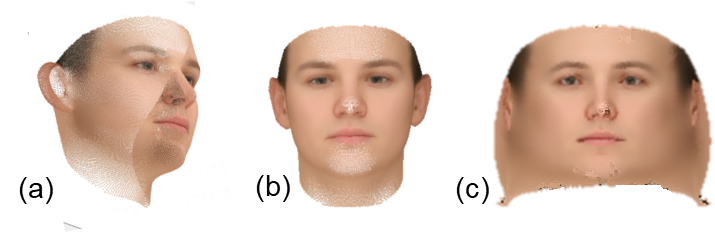
\includegraphics[trim=0 0 0 0,clip, width=0.85\linewidth]{img/tex.png}
\vspace{-3mm}
\caption{\small Three texture representations. (a) Texture value per vertex, (b) Texture as a 2D frontal face, (c) 2D unwarped texture.}
\label{fig:tex_representation}
\figvspace 
\end{figure}

\SubSubSection{Shape \& Texture Representation}
Our shape representation is the same as that of the linear 3DMM, i.e., $\mathbf{S}\in\mathbb{R}^{3\times Q}$ is a set of $Q$ vertices $ \mathbf{v}_S = (x,y,z)$ on the face surface. 
%
The shape decoder $D_S$ is a MLP whose input is the shape parameter $\mathbf{f}_S$ from $E$.

Fig.~\ref{fig:tex_representation} illustrates three possible texture representations. % that could be used for texture. 
Texture is defined per vertex in the linear 3DMM and recent work such as~\cite{tewari2017mofa} (Fig.~\ref{fig:tex_representation}(a)). 
There is a texture intensity value corresponding to each vertex in the face mesh. 
%
Since 3D vertices are not defined on a 2D grid, this representation will be parameterized as a vector, which not only loses the spatial relation of vertices, but also prevents it from leveraging the convenience of deploying CNN on 2D imagery.
%
In contrast, given the rapid progress in image synthesis, it is desirable to choose a 2D image, e.g., a frontal-view face image in Fig.~\ref{fig:tex_representation}(b), as a texture representation. 
%
However, frontal faces contain little information of two sides, which would lose much texture information for side-view faces.

In light of these considerations, we use an unwrapped 2D texture as our texture representation (Fig.~\ref{fig:tex_representation}(c)).
Specifically, each 3D vertex $\mathbf{v}_S$  is projected onto the UV space using cylindrical unwarp. 
Assuming that the face mesh has the top pointing up the $y$ axis, the projection of $\mathbf{v}_S = (x, y, z)$ onto the UV space $\mathbf{v}_T = (u, v)$ is computed as:
\begin{equation}
 v \rightarrow \alpha_1 . \text{arctan} \left( \frac{x}{z} \right) + \beta_1, \hspace{3mm} u \rightarrow \alpha_2 . y + \beta_2,
 \label{eqn:unwarp}
\end{equation}
where $\alpha_1, \alpha_2, \beta_1, \beta_2$ are constant scale and translation scalars to place the unwrapped face into the image boundaries.
Also, the texture decoder $D_T$ is a CNN constructed by fractionally-strided convolution layers. 


\SubSubSection{In-Network Face Rendering}
\label{sec:rendering}

\begin{figure}[t!]
\centering
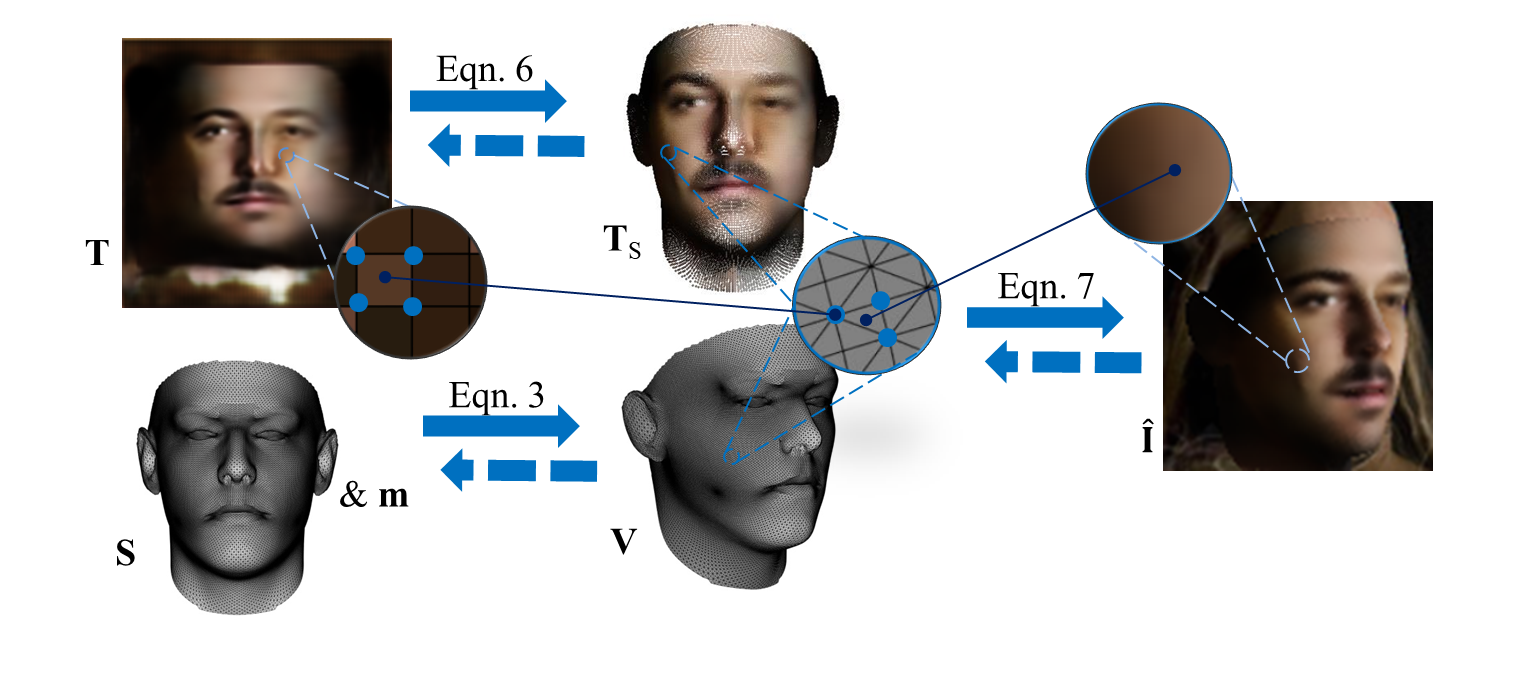
\includegraphics[trim=39 30 35 0,clip, width=0.9\linewidth]{img/Rendering.png}
\vspace{-3mm}
\caption{\small Forward and backward pass of the rendering layer.}
\label{fig:structure}
\figvspace 
\end{figure}

To reconstruct a face image from the texture $\mathbf{T}$, shape $\mathbf{S}$, and projection parameter $\mathbf{m}$, we define a rendering layer $\mathcal{R}(\mathbf{m},\mathbf{S},\mathbf{T})$. %  to render a face image from the above parameters. 
This is accomplished in three steps. 
Firstly, the texture value of each vertex in $\mathbf{S}$ is determined by its predefined location in the 2D texture $\mathbf{T}$. 
Usually, it involves sub-pixel sampling via a bilinear sampling kernel:
\noindent \resizebox{ 0.98\linewidth}{!}{
\begin{minipage}{\linewidth}
\begin{eqnarray}
\mathbf{T}_S(\mathbf{v}_S) = \! \! \! \sum_{ \substack{ u' \in \{ \floor{u}, \ceil{u} \} \\ v' \in \{ \floor{v}, \ceil{v} \} }} \! \! \! \mathbf{T}(u',v')(1{-}|u{-}u'|) (1{-}|v{-}v'|),
\end{eqnarray}
\end{minipage}
}
where $\mathbf{v}_T = (u, v)$ is the UV space projection of $\mathbf{v}_S$ via Eqn.~\ref{eqn:unwarp}.
Secondly, the 3D shape/mesh $\mathbf{S}$ is projected to the image plane via Eqn.~\ref{eqn:projection}.
Finally, the 3D mesh is then rendered using a Z-buffer renderer, where each pixel is associated with a single triangle of the mesh,
\begin{align}
\mathbf{\hat{I}}(m, n) & = \mathcal{R}(\mathbf{m},\mathbf{S}, \mathbf{T})_{m,n}  &= \! \! \! \sum_{\mathbf{v}_S \in \Phi(g, m, n) } \! \! \! \lambda \mathbf{T}_S(\mathbf{v}_S), 
%V & = M \ast S,
\end{align}
where $\Phi(g, m, n) = \{\mathbf{v}_S ^{(1)}, \mathbf{v}_S ^{(2)}, \mathbf{v}_S^{(3)} \}$ is an operation returning three vertices of the triangle that encloses the pixel $(m, n)$ after projection $g$. 
In order to handle occlusions, when a single pixel resides in more than one triangle, the triangle that is closest to the image plane is selected. 
The value of each pixel is determined by interpolating the intensity of the mesh vertices via barycentric coordinates $\{\lambda^{(i)}\}_{i=1}^3$.

There are alternative designs to our rendering layer. 
If the texture representation is defined per vertex, as in Fig.~\ref{fig:tex_representation}(a), one may warp the input image $\mathbf{I}_i$ onto the vertex space of the 3D shape $\mathbf{S}$, whose distance to the per-vertex texture representation can form a reconstruction loss. 
This design is adopted by the recent work of~\cite{tewari2017mofa}.
In comparison, our rendered image is defined on a 2D grid while the alternative is on top of the 3D mesh.
As a result, our rendered image can enjoy the convenience of applying the adversarial loss, which is shown to be critical in improving the quality of synthetic texture.
%Further, our 2D texture representation can be generated through convolutional filters, which substantially reduces the number of parameters in $D_T$.
%
Another design for rendering layer is image warping based on the spline interpolation, as in~\cite{cole2017face}. 
However, this warping is continuous: every pixel in the input will map to the output. 
Hence this warping operation fails in the occlusion part. 
As a result, Cole et al.~\cite{cole2017face} limit their scope to only synthesizing frontal faces by warping from normalized faces. \footnote{Our rendering layer implementation is publicly available at~\url{https://github.com/tranluan/Nonlinear_Face_3DMM}.}

\begin{table}[t!]
\caption{\small The structures of $E$ and $D_T$ networks}
\vspace{-6mm}
\label{tab:network}
%\figvspace 
\begin{center}
\small
\resizebox{0.99\linewidth}{!}{
\setlength{\tabcolsep}{3pt}
\begin{tabular}{ @{}ccccccccc@{} }
\toprule
\multicolumn{3}{c}{$E$} & \hspace{2mm} 
& \multicolumn{3}{c}{$D_T$} \\
\cmidrule(r){1-3}
\cmidrule(r){5-7}
Layer & Filter/Stride & Output Size && Layer & Filter/Stride & Output Size \\ \midrule
&&&& FC & & $8{\times}8{\times}320$ \\
Conv11 & $3{\times}3/1$ & $96{\times}96{\times}32$ && FConv52& $3{\times}3/1$ & $8{\times}8{\times}160$ \\
Conv12 & $3{\times}3/1$ & $96{\times}96{\times}64$ && FConv51& $3{\times}3/1$ & $8{\times}8{\times}256$ \\\midrule
Conv21 & $3{\times}3/2$ & $48{\times}48{\times}64$ && FConv43& $3{\times}3/2$ & $16{\times}16{\times}256$&&\\ 
Conv22 & $3{\times}3/1$ & $48{\times}48{\times}64$  && FConv42& $3{\times}3/1$ & $16{\times}16{\times}128$ \\
Conv23 & $3{\times}3/1$ & $48{\times}48{\times}128$ && FConv41& $3{\times}3/1$ & $16{\times}16{\times}192$ \\
\midrule
Conv31 & $3{\times}3/2$ & $24{\times}24{\times}128$ && FConv33& $3{\times}3/2$ & $32{\times}32{\times}192$ && \\ 
Conv32 & $3{\times}3/1$ & $24{\times}24{\times}96$  && FConv32& $3{\times}3/1$ & $32{\times}32{\times}96$ \\
Conv33 & $3{\times}3/1$ & $24{\times}24{\times}192$ && FConv31& $3{\times}3/1$ & $32{\times}32{\times}128$ \\
\midrule
Conv41 & $3{\times}3/2$ & $12{\times}12{\times}192$ && FConv23& $3{\times}3/2$ & $64{\times}64{\times}128$ \\ 
Conv42 & $3{\times}3/1$ & $12{\times}12{\times}128$ && FConv22& $3{\times}3/1$ & $64{\times}64{\times}64$ \\
Conv43 & $3{\times}3/1$ & $12{\times}12{\times}256$ && FConv21& $3{\times}3/1$ & $64{\times}64{\times}64$ \\
\midrule
Conv51 & $3{\times}3/2$ & $6{\times}6{\times}256$ && 
FConv13& $3{\times}3/2$ & $128{\times}128{\times}64$ \\ 
Conv52 & $3{\times}3/1$ & $6{\times}6{\times}160$ && FConv12& $3{\times}3/1$ & $128{\times}128{\times}32$ \\
Conv53 & $3{\times}3/1$ & $6{\times}6{\times}(l_S{+}l_T{+}64)$ && FConv11& $3{\times}3/1$ & $128{\times}128{\times}3$ \\
\midrule
AvgPool& $6{\times}6/1$ & $1{\times}1{\times}(l_S{+}l_T{+}64)$ && \\ \midrule
FC (for $\mathbf{m}$ only) & $64{\times}6$& $6$ \\ \bottomrule
\end{tabular}}
\vspace{-6mm}
\end{center}
\end{table}


\SubSubSection{Network Architecture}
We design our $E, D_T$ network architecture as in Tab.~\ref{tab:network}. Also, $D_S$ includes two fully connected layers with \mbox{$1,000$-dim} intermediate representation with eLU activation.

The entire network is end-to-end trained to reconstruct the input images, with the loss function:
\begin{equation}
L = L_{\text{rec}} + \lambda_{ \text{adv} } L_{ \text{adv} } +  \lambda_L L_{\text{L}},
\label{tab:overallLoss}
\end{equation}
where the reconstruction loss $L_{\text{rec}} = \sum_{i=1}^{N}||\mathbf{\hat{I}}_i - \mathbf{I}_i||_1$ enforces the rendered image $\mathbf{\hat{I}}_i$ to be similar to the input $\mathbf{I}_i$, the adversarial loss $L_{ \text{adv} }$ favors realistic rendering, and the landmark loss $L_L$ enforces geometry constraint.

\Paragraph{Adversarial Loss}
Based on the principal of Generative Adversarial Network (GAN)~\cite{goodfellow2014generative}, the adversarial loss is widely used to synthesize photo-realistic images~\cite{radford2015unsupervised, tran2017disentangled, tran2018representation}, where the generator and discriminator are trained alternatively.
In our case, networks that generate the rendered image $\mathbf{\hat{I}}_i$ is the generator.
The discriminator includes a dedicated network $D_A$, which aims to distinguish between the real face image $\mathbf{I}_i$ and rendered image $\mathbf{\hat{I}}_i$.
During the training of the generator, the texture model $D_T$ will be updated with the objective that $\mathbf{\hat{I}}_i$ is being classified as real faces by $D_A$.
%
Since our face rendering already creates correct global structure of the face image, the global image-based adversarial loss may not be effective in producing high-quality textures on local facial regions.
Therefore, we employ patchGAN~\cite{shrivastava2017learning} in our discriminator.
%
Here, $D_A$ is a CNN consisting of four $3\times3$ conv layers with stride of $2$, and number of filters are $32$, $64$, $128$ and $1$, respectively. 
%
Finally, one of key reasons we are able to employ adversarial loss is that we are rendering in the 2D image space, rather than the 3D vertices space or unwrapped texture space.
This shows the necessity and importance of our rendering layer. 
 
\Paragraph{Semi-Supervised Pre-Training}  
Fully unsupervised training using only the mentioned reconstruction and adversarial loss on the rendered image could lead to a degenerate solution, since the initial estimation is far from ideal to render meaningful images. 
Hence, we introduce pre-training loss functions to guide the training in the early iterations.

With face profiling technique, Zhu et al.~\cite{zhu2016face} expands the 300W dataset~\cite{sagonas2016300} into $122,450$ images with the fitted 3DMM shape $\widetilde{\mathbf{S}}$ and projection parameters $\widetilde{\mathbf{m}}$. 
Given $\widetilde{\mathbf{S}}$ and $\widetilde{\mathbf{m}}$, we create the pseudo groundtruth texture $\widetilde{\mathbf{T}}$ by referring every pixel in the UV space back to the input image, i.e., backward of our rendering layer. 
With $\widetilde{\mathbf{m}}$, $\widetilde{\mathbf{S}}$, $\widetilde{\mathbf{T}}$, we define our pre-training loss by: 
\begin{equation}
L_0 = L_{\text{S}} + \lambda_T L_{\text{T}} + \lambda_m L_{\text{m}} + \lambda_L L_{\text{L}},
\end{equation}
where
\begin{align}
L_{\text{S}} = & \norm{ \mathbf{S}-\mathbf{\widetilde{S}} }_2, \\
L_{\text{T}} = & \norm{ \mathbf{T}-\mathbf{\widetilde{T}} }_1, \\
L_{\text{m}} = & \norm{ \mathbf{m}-\mathbf{\widetilde{m}} }_2. 
\end{align}
% $L_{\text{S}} =  ||\mathbf{S}-\mathbf{\widetilde{S}} ||_2$, $L_{\text{T}} =  || \mathbf{T}-\mathbf{\widetilde{T}} ||_1$, and $L_{\text{m}} =  || \mathbf{m}-\mathbf{\widetilde{m}} ||_2$.
Due to the pseudo groundtruth, using $L_0$ may run into the risk that our solution learns to mimic the linear model. 
Thus, we switch to the loss of Eqn.~\ref{tab:overallLoss} after $L_0$ converges.

\Paragraph{Sparse Landmark Alignment}
To help $D_T$ to better learn the facial shape, the landmark loss can be an auxiliary task. 
\begin{align}
L_{\text{L}} = & \norm {M(\mathbf{m}) \ast \begin{bmatrix} \mathbf{S}(:,\mathbf{d}) \\ \mathbf{1} \end{bmatrix} - \mathbf{U} }_2,
\label{eq:landmarkloss}
\end{align}
where $\mathbf{U} \in \mathbb{R}^{2{\times} 68}$ is the manually labeled 2D landmark locations, $\mathbf{d}$ is a constant $68$-dim vector storing the indexes of $68$ 3D vertices corresponding to the labeled 2D landmarks.
Unlike the three losses above, these landmark annotations are ``golden" groundtruth, and hence $L_{\text{L}}$ can be used during the entire training process. 
Different from traditional face alignment work where the shape bases are fixed, our work jointly learns
the bases functions (i.e., the shape decoder $D_S$) as well. 
Minimizing the landmark loss when updating $D_S$ only moves a tiny subset of vertices, since our $D_S$ is a MLP consisting of fully connected layers.
This could lead to unrealistic shapes. 	
Hence, when optimizing the landmark loss, we fix the decoder $D_S$ and only update the encoder.
Note that the estimated groundtruth in $L_0$ and the landmarks are the only supervision used in our training, due to this our learning is considered as {\it weakly} supervised. 
